\documentclass[10pt,a4paper]{article}

% change to german
\usepackage[german]{babel}

% better hyphenation
\usepackage[final]{microtype}
\usepackage{csquotes}

% packages, images, math
\usepackage{geometry, graphicx, amsmath, amsfonts, array, multicol, multirow}

% bar charts
\usepackage{bchart}

% for bibliography
\usepackage[
    backend=biber,
    style=alphabetic,
    sorting=ynt,
    minalphanames=3,
]{biblatex}
\addbibresource{./references.bib}

% import line spacing
\usepackage{setspace}

% colors
\usepackage{xcolor}

% for urls
\usepackage[colorlinks=true, urlcolor=blue, citecolor=blue, linkcolor=black]{hyperref}

% Remove Indentation at new line
\setlength{\parindent}{0cm}

% Set Font to Arial, needs xelatex
% \usepackage{fontspec}
% \setmainfont{Arial}

% Set Font to Helvet
\usepackage{helvet}
\renewcommand{\familydefault}{\sfdefault}

% Set Layout
\geometry{
    a4paper,
    left=25mm,
    right=25mm,
    top=25mm,
    bottom=20mm
}

% Redefine title
\makeatletter
\def\@maketitle{%
  \newpage
  \null
  \vskip 2em%
  \begin{center}%
  \let \footnote \thanks
    {\Huge\bfseries\@title \par}%
    \vskip 1.5em%
    {\large
      \lineskip .5em%
      \begin{tabular}[t]{c}%
        \@author
      \end{tabular}\par}%
    \vskip 1em%
    {\large \@date}%
\end{center}%
\par
\vskip 1.5em}
\makeatother

% set line spacing
\setstretch{1.25}

% document
\begin{document}

\title{Supersonic Algorithms}
\author{Anton Rodenwald}

\maketitle

\large\begin{tabular}{l p{12cm}}

    Projektbetreuerin: & Birgit Ziegenmeyer \\

    Institution: & Schillerschule Hannover \\
    
    Thema des Projektes: 
    & Analyse verschiedener Implementationen von Algorithmen 
    in Bezug auf die besten Techniken zur Optimierung 
    und Auseinandersetzung mit der Ausführung dieser,
    um die Umsetzung hochperformanter und effizienter
    Programme zu erforschen. \\

    Fachgebiet: & Mathematik/Informatik \\

    Wettbewerbssparte: & Jugend Forscht \\
    
    Bundesland: & Niedersachsen \\
    
    Wettbewerbsjahr: & 2023 \\
    
\end{tabular}

\clearpage

\begin{bchart}
    \bcbar{1.4}
\end{bchart}

\section*{Kurzfassung}

Nachdem wir im Informatikunterricht der SEK II Sortieralgorithmen behandelt hatten,
stellte ich mir die Frage, wie man am schnellsten eine Liste von 10 Millionen zufällig Generierten Zahlen
sortieren kann und welche Programmiersprache und welche Techniken man nutzen sollte.
Daraus entwickelte sich dann die etwas allgemeinere Fragestellung, 
nämlich welche Optimierungen erhöhen die Ausführgeschwindigkeit von Programmen am meisten und wieso?
Im breiteren Kontext gesehen ist diese Fragestellung wichtig, weil die schnelle Ausführung von Programmen aller Art
zur Einsparung von monetären und natürlichen Ressourcen führt und somit konkret bei Unternehmen den Gewinn
vervielfachen kann oder vor allem in großen Rechenzentren Energie sparen kann.
Mir war bekannt, dass Python, was wir im Unterricht verwendet hatten, als eine der langsamsten Sprachen gilt, 
weswegen ich neben Python auch noch C++ wählte, was allgemein als eine der schnellsten Sprachen gilt.
Ich implementierte anschließend verschiedene Variationen der Quicksort und anderer Algorithmen und testete so, 
in welchem Maß Optimierungsansätze die Performance beeinflussten.
Dabei kam ich zu dem Ergebnis, dass die besten Python-Bibliotheken zur Optimierung NumPy und Numba waren,
womit die Performance gleich zu der in C++ war.
Dies erklärte ich mir dadurch, dass Python und C++ zwar durchaus verschieden sind, aber es in Python möglich ist, C/C++ Funktionen zu
nutzen, womit diese bei vielen Aufgaben gleichzusetzen sind.
Schlussendlich gelang es mir noch unter Nutzung von AVX2, einem speziellen Befehlssatz von Intel, und dem Radixsort Algorithmus eine 4x schnellere Version als die standardmäßig 
Vorhande in C++ zu implementieren, was mir zeigte, dass es im Gebiet der Codeoptimierung noch immer Möglichkeiten zur Optimierung gibt
und nicht immer alles schon so schnell wie möglich implementiert ist.

\clearpage

\renewcommand*\contentsname{Inhaltsverzeichnis}

\tableofcontents

\clearpage

\section{Einleitung}

Im Informatik Leistungskurs des 12. Jahrgangs beschäftigten wir uns nach den Herbstferien mit
der Laufzeit von Algorithmen am Beispiel der Quicksort, einem Sortieralgorithmus.
Nach diesem thematischen Impuls ergab sich mein Projekt zur Erforschung von Sortieralgorithmen,
in dem ich es mir zuerst zur Aufgabe gemacht hatte, den schnellsten Weg zu finden, 10 Millionen zufällig
generierte Zahlen zu sortieren. Mein Fokus änderte sich dann allerdings und ich fokussierte mich
auf die Aspekte der Implementation und tatsächlichen Ausführung der Programme, da 
Sortieralgorithmen algorithmisch bereits sehr weit erforscht sind und man in diesem Gebiet nur
sehr schwer neue Erkenntnisse sammeln konnte \cite{sortieralgorithmenwikipedia}.
Ich entschied mich deswegen, nicht nach besseren Algorithmen zu suchen, sondern nach Wegen, 
mein ursprüngliches Programm in Python in seiner Ausführung zu beschleunigen und so vorteilhafte
Wege der Geschwindigkeitsoptimierung zu entdecken.
Ich stellte mir die Frage, welche Optimierungen die Ausführgeschwindigkeit von Programmen
am meisten erhöhen und wieso?
Zum Thema der Optimierung fand ich in Bezug auf Python einige Bibliotheken im Internet, die
bessere Performance versprachen, von denen ich einige auswählte, um herauszufinden,
welche dieser den größten Geschwindigkeitsboost bringt.
Außerdem entschied ich mich noch dazu, einige Algorithmen auch in C++ zu implementieren, wobei ich in Bezug
darauf nicht direkt Möglichkeiten und Erklärungen fand, welche Modifikationen ein Programm schneller machen und
wieso diese Veränderungen es schneller machen.
Weiterführend verglich ich noch, wie sich meine C++ Programme mit denen in Python in der Ausführung auf einer
tiefergreifenden Stufe unterschieden, um herauszufinden, wieso C++ größtenteils deutlich schneller ist.
Meine Erwartung war dabei, dass C++ bei jeder Aufgabe Python um ein Vielfaches übertrifft, vor allem im Punkt der Geschwindigkeit,
da Python im Allgemeinen als langsam gilt und C++ als sehr performant und schnell.

\clearpage

\section{Vorgehensweise, Materialien, Methode}

\subsection{Vorgehen}

Meine Vorgehensweise beruhte darauf, mich im Internet über Möglichkeiten der Optimierung zu informieren und diese geschickt neu zu kombinieren und die erreichten Geschwindigkeiten miteinander zu vergleichen, wodurch
ich eine qualitative Entscheidung treffen konnte, welche Variationen die größten Performanceverbesserungen bringen.
Dazu wählte ich die Python-Bibliotheken NumPy, Numba, CTypes und Cython und
testete auch Funktionen aus den Standardbibliotheken der Sprachen.
Bei der Implementation nutzte ich Internetquellen wie Stackoverflow, die Cython Dokumentation und andere 
(alle Seiten aufzuzählen ist nicht zielführend), um die Implementierung umzusetzen, 
da ich noch kaum Erfahrung mit diesen Bibliotheken hatte \cite{stackoverflow} \cite{cythondocs}.
Dies wurde besonders wichtig beim Implementieren in den mir noch kaum bekannten Sprachen Java, Lua, Julia und Go.
Meine Implementationstechnik war das iterative Implementieren, wo ich eine Startversion immer wieder abwandelte und
fortlaufend Dinge änderte. Dabei behielt ich immer die Ausführungszeit im Auge und entschied so, welche Ansätze
weitere Tests erforderten.
Bei der Implementation einer Radixsort, einem sehr schnellen Sortierverfahren, nutze ich außerdem 2 Publikationen 
zur Verbesserung meiner eigenen Variante und schuf so die Untergrenze all meiner getesteten Implementationen
\cite{terdiman} \cite{michael}.
Im Zuge dessen beschäftigte ich mich auch mit dem Konzept von AVX2 und nutze diesen erweiterten Befehlssatz, den
ich im Rahmen der Ergebnisse noch weiter beschreiben werde.
\cite{intelavxdocs} \cite{avxguide}.

\clearpage

\subsection{Materialien}
Für mein Projekt nutze ich meinen Desktop PC (Linux) und meinen Laptop (Linux) zur Implementation und Ausführung der Programme.
Dabei nutze ich verschiedene Arten von Software zum Entwickeln und Ausführen meiner Programme und zum Erstellen meiner
schriftlichen Arbeit. \newline

Ich nutze dabei diese Software in der jeweiligen Version:

\begin{itemize}
    \item clang++ 14.0.6 (C/C++ Compiler)
    \item python 3.10.8 (Ausführen der Dateien)
    \item java 19.0.1 openjdk (Javac, JVM)
    \item lua 5.4.4 (Ausführen der Dateien)
    \item nodejs 18.8.0 (Ausführen der Dateien)
    \item julia 1.8.3 (Ausführen der Dateien)
    \item go 1.19.4 (Kompilierung)
\end{itemize}

\subsection{Methode}

Meine Methode war das strukturierte Testen und Vergleichen von Programmimplementationen und ihrer 
Variationen mithilfe einer einfachen Zeitnahme. Ich nutze die Möglichkeiten der jeweiligen Programmiersprachen, 
um die Ausführungszeiten auf die Millisekunde genau oder sogar genauer zu bestimmen und 
so zu vergleichen zu machen. In Python definierte ich mir dafür eine eigene Klasse (Abb. 1), fügte das Starten und Stoppen
des Timers meinem Code hinzu (Abb. 2) und ließ mir die Ergebnisse als Text ausgeben (Abb. 3).
Damit die Ergebnisse vergleichbar sind, implementierte ich immer auf ähnliche Weise die Algorithmen und
nutze die gleichen Eingabewerte und Konstanten.
Als Beispiel generierte ich mir in jeder Sprache eine Liste aus 10 Millionen Zufallszahlen,
was ich nicht in die Zeit mit einbezog, und wendete auf diese dann die implementierten Algorithmen an.
So hatten alle Programme die gleiche Aufgabe zu lösen, wodurch Vergleichbarkeit gewährleistet ist.
Wichtig war auch, die finalen Tests direkt nach einem Neustart des PCs ohne andere laufende Programme
zu machen, damit es durch variierende Prozessorauslastung keine Verfälschungen gab. 

% \begin{multicols}{2}
    
% \end{multicols}

\begin{center}
    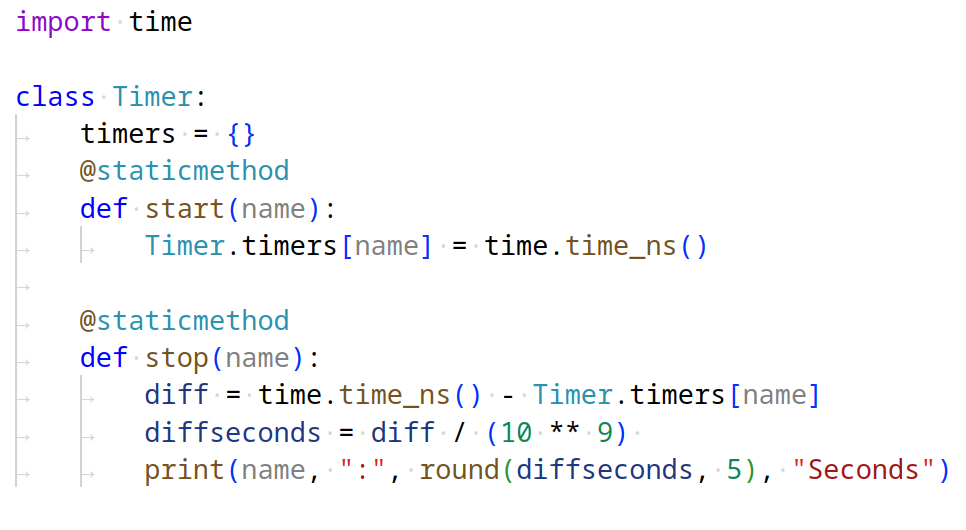
\includegraphics[width=0.75\textwidth]{screenshots/pythontimerlight.png}
    
    Abb. 1 Timer Klasse
\end{center}

\begin{center}
    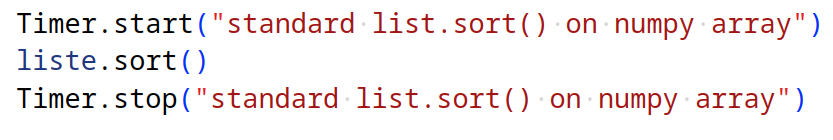
\includegraphics[width=.75\textwidth]{screenshots/timerexamplelight.png}
    
    Abb. 2 Nutzungsbeispiel
    
    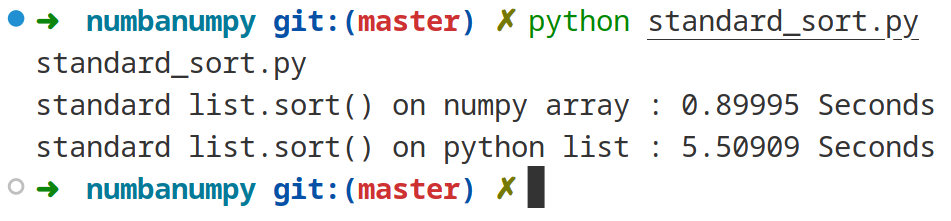
\includegraphics[width=.75\textwidth]{screenshots/outputexamplelight.png}

    Abb. 3 Beispielausgabe
\end{center}

\subsection{Schwierigkeiten}

Die größte Schwierigkeit war, dass ich auf diesem Themengebiet noch nicht sehr viel Vorerfahrung hatte.
Außerdem waren die Konzepte teils komplex und es war nicht immer einfach, im Internet gute Beispiele zur Implementierung
zu finden. Vor dem Projekt hatte ich mich z. B. noch nie mit der Python Bibliothek "ctypes" beschäftigt und deshalb fand
ich meist erst nach längerem Suchen im Internet eine Lösung für auftretende Fehler.
Auch bei der Implementation von Programmen in C++ hatte ich teils meine Schwierigkeiten, da das Verstehen
von einigen Bitoperationen erstmal ein Eindenken in die Thematik erforderte.
Mit dem Ausführen der Programme hatte ich hingegen kaum Probleme.
Ein für mich nicht lösbares Problem war auch die Implementierung in Go, wo nur das Generieren
einer 7 Millionen Zahlen langen Liste möglich, da bei mehr Zahlen mehr Arbeitsspeicher benötigt wurde,
als Go in einem Programmteil erlaubt. Der hohe Verbrauch an Arbeitsspeicher kommt meinen Vermutungen
nach von der Implementation von Rekursion in Go, die nicht für sehr tiefe Rekursion geeignet scheint
\cite{godeeprecursions} \cite{goroutinesize}.

\clearpage

\section{Ergebnisse}

\subsection{Zufallzahlengenerierung}

\begin{center}
    \hspace*{-1.5cm}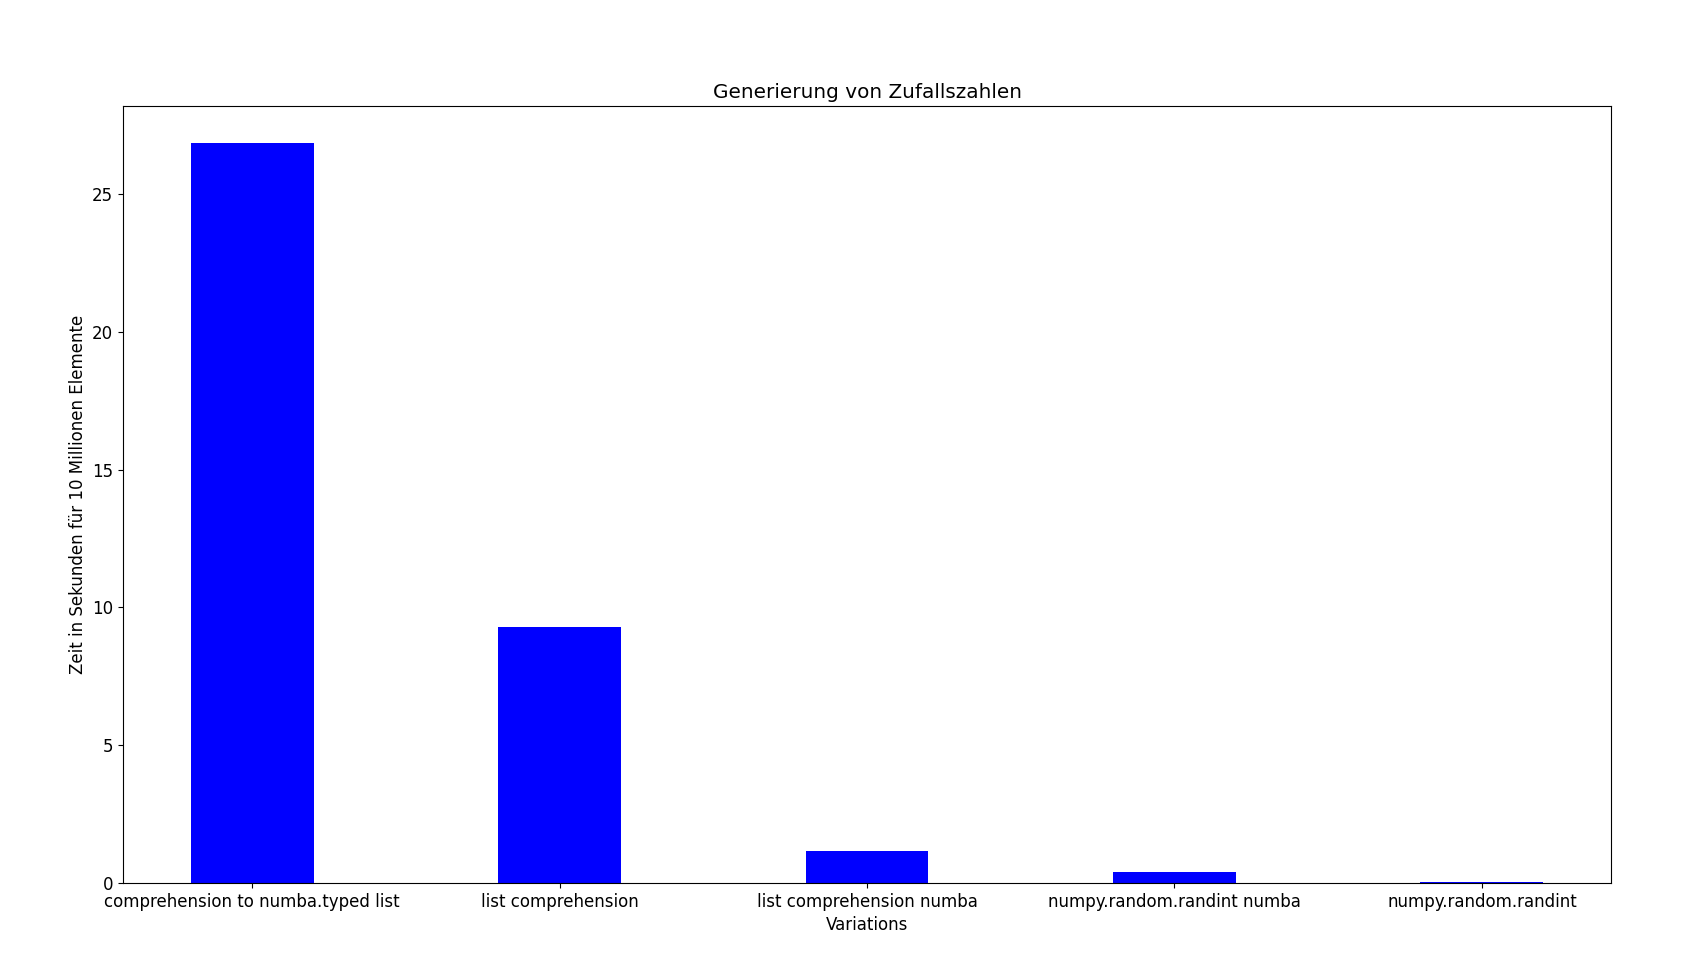
\includegraphics[width=1.2\textwidth]{./diagramme/matplotlib/zufallszahlen.png}
    Abb. 4 Zufallszahlengenerierung
\end{center}

Zuerst beschäftigte ich mich damit, möglichst schnell die Liste von Zufallszahlen zu generieren.
Die nicht optimierten Version, die reine "List Comprehensions" nutzen, schneiden erwartungsgemäß schlecht ab
und sind deutlich langsamer als andere Varianten. Die Numba nutzende Version ist ca. 5x schneller,
was darauf zurückzuführen ist, dass der ursprüngliche Python Code dem Numba JIT-Compiler übergeben wird.
JIT Compilation bedeutet, dass während des Ausführens des Programms Teile des Programms wie z. B. Funktionen
vom JIT-Compiler in eine optimierte Form zur Ausführung übertragen werden. Dies kostet zwar Zeit, doch bei
Funktionen, die häufig ausgeführt werden oder wenn die Optimierungen eine sehr große Zeitersparnis bringen.
Der 2. Aspekt ist hier der Fall, obwohl die Kompilierung Zeit kostet, wird diese bei der Ausführung deutlich eingespart.
Schneller sind nur die Funktion "numpy.random.randint, die ein NumPy Array mit Zufallszahlen erstellt,
wobei hier auffällt, dass diese durch den JIT-Compiler nicht schneller wird, was damit zusammenhängt, dass die Kompilierung
länger als die eigentliche Ausführung dauert. Die Erklärung dafür, dass diese Funktion der NumPy Bibliothek
so schnell ist, ist darin zu finden, dass diese in C geschrieben wurde und bereits kompiliert wurde. Dadurch wird
das NumPy Array genauso schnell wie in C generiert. Diese fand ich durch Betrachten des NumPy Github Repository heraus.

\subsection{Langsame Implementatin in Python/Cython}

\begin{center}
    \hspace*{-1.5cm}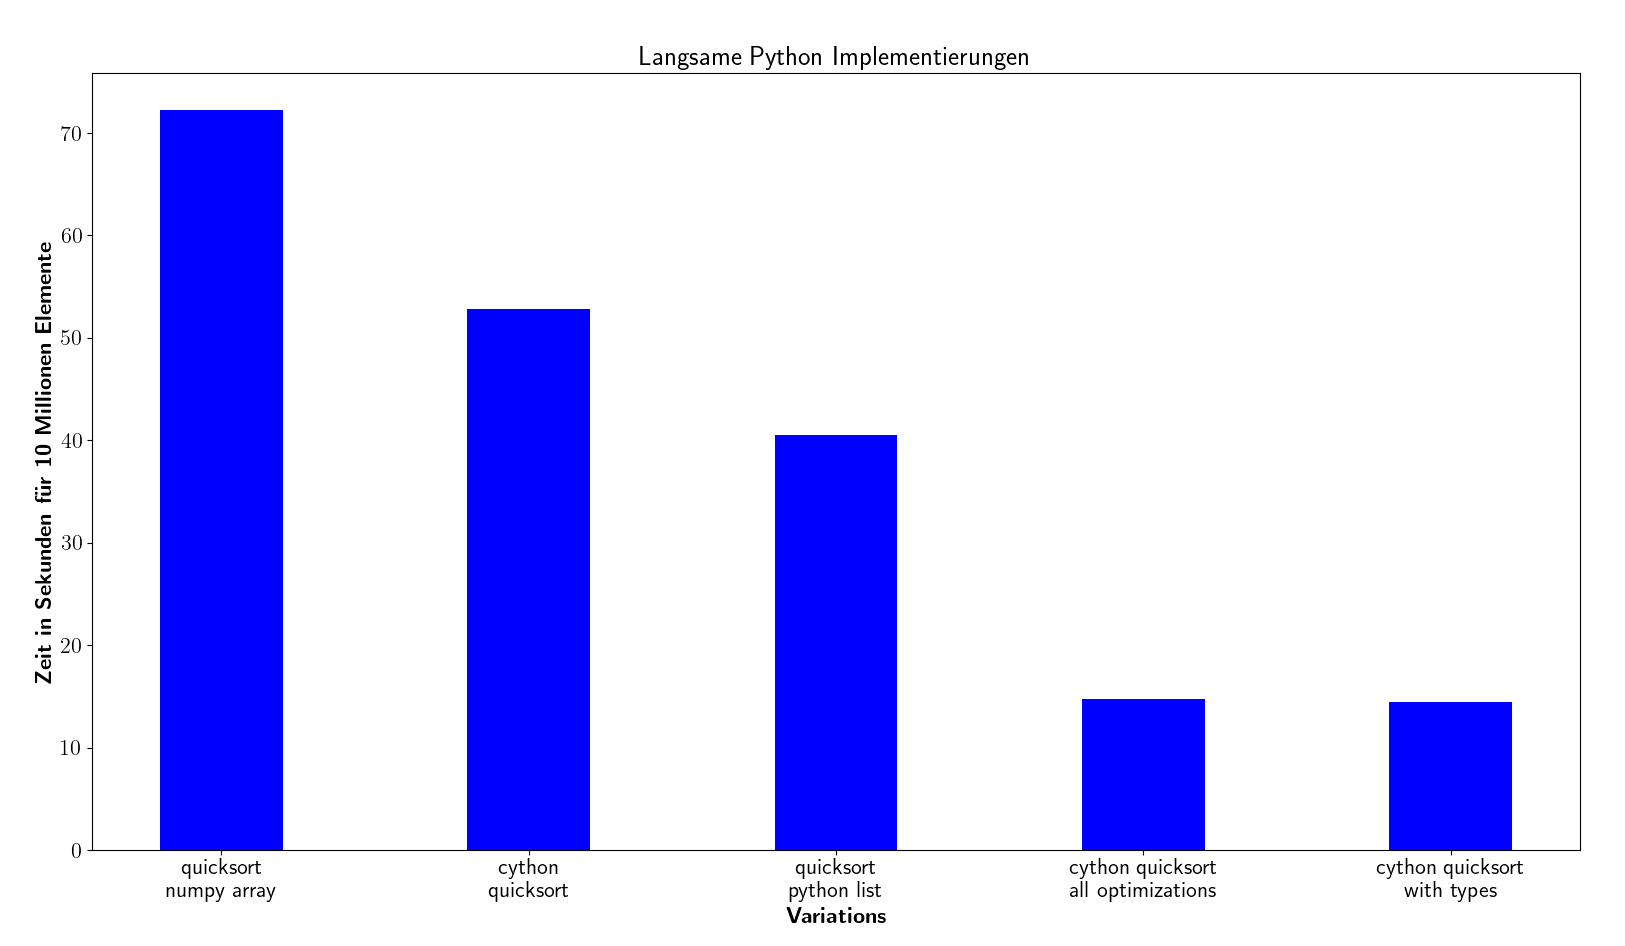
\includegraphics[width=1.2\textwidth]{./diagramme/matplotlib/pythonlangsam.png}
    Abb. 5 Schlechte Performance
\end{center}

Nachdem nun eine zu sortierende Liste vorhanden war, implementierte ich mehrere Versionen der Sortieralgorithmen.
In Abbildung 5 sind die langsamen Versionen zu sehen, bei denen wenige Optimierungen vorgenommen wurden, oder wo diese nichts bewirkten.
Ausgehend von der Implementation mit normalen Python-Listen reduzierte sich die Ausführdauer von ca. 40 auf 14 Sekunden
durch die Nutzung von statischer Typisierung und Kompilierung mit Cython. Das hinzufügen weiteres Optimierungen
bei Cython (all optimizations) hatte in diesem Fall dann allerdings keine Auswirkungen mehr.
Zu erklären ist die um 281\% höhere Geschwindigkeit damit, dass der Cython Code vom Cython Compiler
entsprechend kompiliert werden kann und die in Cython implementierten Funktionen somit bereits besser
Optimiert sind bei ihrer Ausführung als normaler Python Code, der mühsam vom Python-Interpreter eingelesen
und verarbeitet werden muss, was mehr Zeit kostet.
Überraschend war für mich, dass das Nutzen von den scheinbar schnelleren NumPy Arrays und das Kompilieren
von reinem Python Code mit Cython für eine Verschlechterung sorgten, was ich mir dadurch erklärte, dass einige
Python Funktionen auf normale Listen besser funktionieren als auf NumPy Arrays, da sich diese in ihrer Funktionsweise
unterscheiden. Warum die Cython Version langsamer ist, konnte ich mir noch nicht erklären, wobei es vielleicht an meinem
noch nicht tiefgreifend genug gehenden Verständnis von Cython liegen könnte oder daran, dass es etwas Zeit kostet,
die mit Cython kompilierten Funktionen aufzurufen

\subsection{Schnelle Implementationen mit NumPy und Numba}

\begin{center}
    \hspace*{-1.5cm}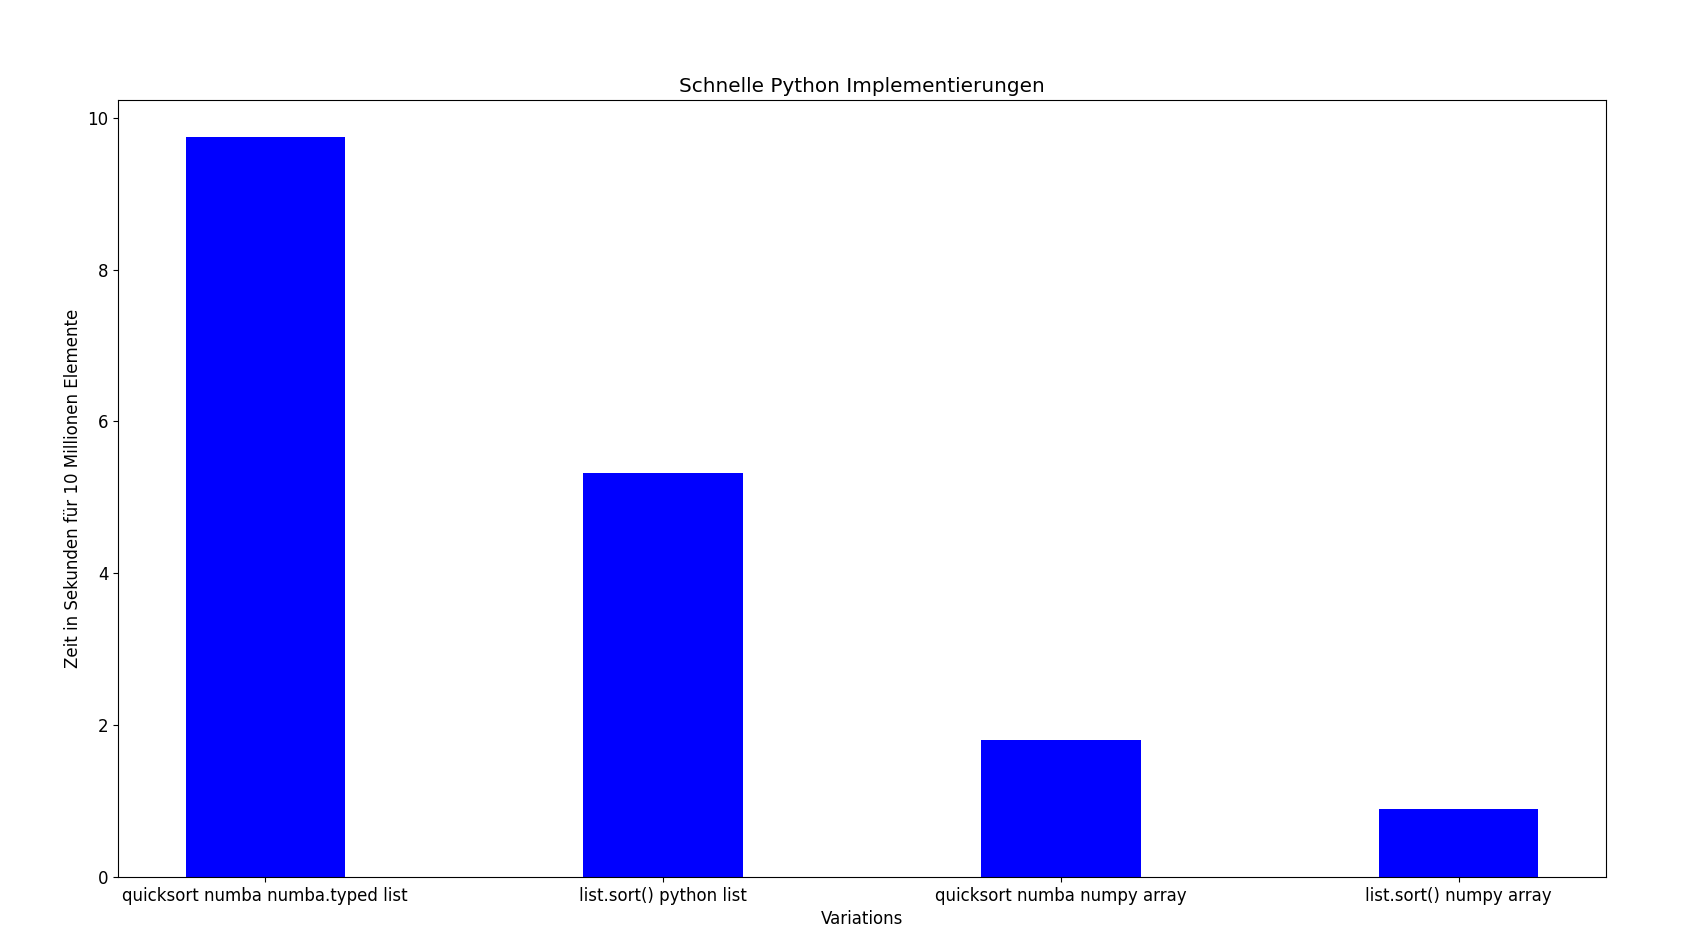
\includegraphics[width=1.2\textwidth]{./diagramme/matplotlib/pythonschnell.png}
    Abb. 6 Schnelle Programme
\end{center}

Deutlich erfolgreicher und einfacher war die Implementierung mit Numba und NumPy.
Es zeigte sich, dass das Anwenden von JIT-Kompilierung in Form von 1er-Zeile Code
eine Reduzierung auf $\approx$ 9 und $\approx$ 2 Sekunden bewirkt. Diese hohe Effektivität von JIT
ist aufgrund dessen, dass die Quicksort Funktion sich häufig rekursiv aufruft, und so bei jedem Aufruf
Zeit eingespart wird, was sich dann aufsummiert zu einer hohen Zeitersparnis.
Außerdem fällt auf, dass die standardmäßig in Python implementierte 'sort()' Methode der Listen
am besten abschneidet. Diese ist nämlich, wie die NumPy Funktionen und alle built-in Python Funktionen, in C geschrieben und
somit sehr schnell. Mit der Kombination der in C geschriebenen Funktionen erreicht man so eine Zeit von 0.9 Sekunden.

\subsection{C++, CTypes und Radixsort}

\begin{center}
    \hspace*{-1.5cm}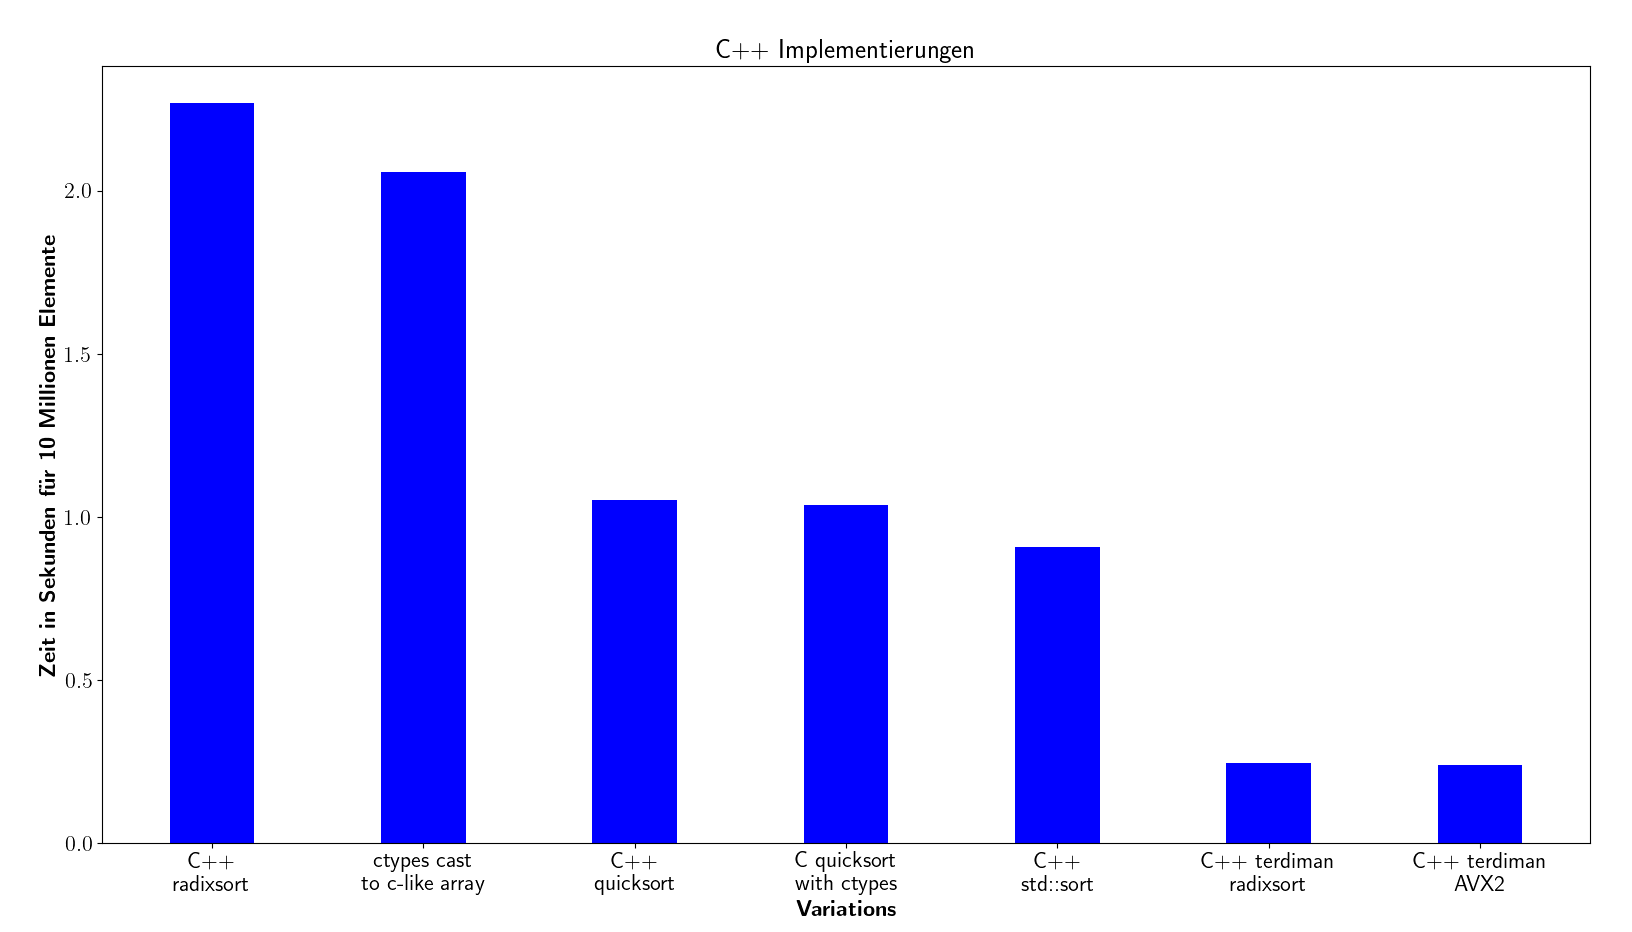
\includegraphics[width=1.2\textwidth]{./diagramme/matplotlib/cpp.png}
    Abb. 7 C/C++ Implementationen
\end{center}

Bei meiner Implementation des Quicksort Algorithmus in C++ und dem Testen der standardmäßigen Sortierfunktion
fiel mir auf, dass diese nahezu gleich schnell waren wie die schnellste Python Implementierung.
Daraus schloss ich, dass kaum ein Unterschied bestand zwischen dem, was der Computer bei meinem C++ Code und beim schnellsten Python Code machte.
Die genutzten Python-Funktionen waren ja schließlich auch in C geschrieben. Diese Vermutung bestätigte ich, indem
ich meine in C++ Quicksort nach C umschrieb und mit dem Modul CTypes aus Python heraus aufrief und damit ähnliche Geschwindigkeiten
erreichte. Es zeigt sich, dass die Geschwindigkeit von Python Code stark davon abhängt, ob Funktionen in C geschrieben wurden,
die man nur noch aufrufen muss, oder ob Funktionen in Python ausgeführt werden müssen.
Abschließend gelang es mir noch, einige weitere Techniken der Optmierung in C++ zu entdecken und umzusetzen.
Meine ursprüngliche Implementation der RadixSort, einem Sortierverfahren der Komplexität $n \cdot w$ , was theoretisch deutlich schneller ist als die Quicksort
mit einer Komplexität von $n \cdot log_{n}$, stellte sich als langsamer als die Versionen  der Quicksort in Python und C++ heraus.
Ich konnte mir erst nicht erklären, wie dies der Fall sein konnte, bis mir durch einen Artikel von Pierre Terdimann Optimierungsmöglichkeiten
aufgezeigt wurden. Ich konnte so eine sehr zentrale, ursprünglich komplexe und kostspielige Operation in meinem Code ersetzen
und so die Geschwindigkeit um das 20-fache erhöhen von $\approx$ 2.2 auf $\approx$ 0.24 Sekunden \cite{terdiman}.
Diese Operation, die zentral zur Bestimmung der schlussendlichen Position der Elemente im sortierten Array ist, konnte ich nun in einem Teil meines Programms noch weiter verbessern und so die Ausführung dieses Programmteils
um insgesamt 5ms reduzieren, nachdem ich durch eine weitere Publikation auf die Idee gebracht wurde, den erweiterten Befehlssatz namens
AVX2 zu nutzen \cite{michael}. Wie genau ich diesen nutzte, werde ich bei der Diskussion weiter ausführen.

\subsection{Sprachenvergleich}

\begin{center}
    \hspace*{-1.5cm}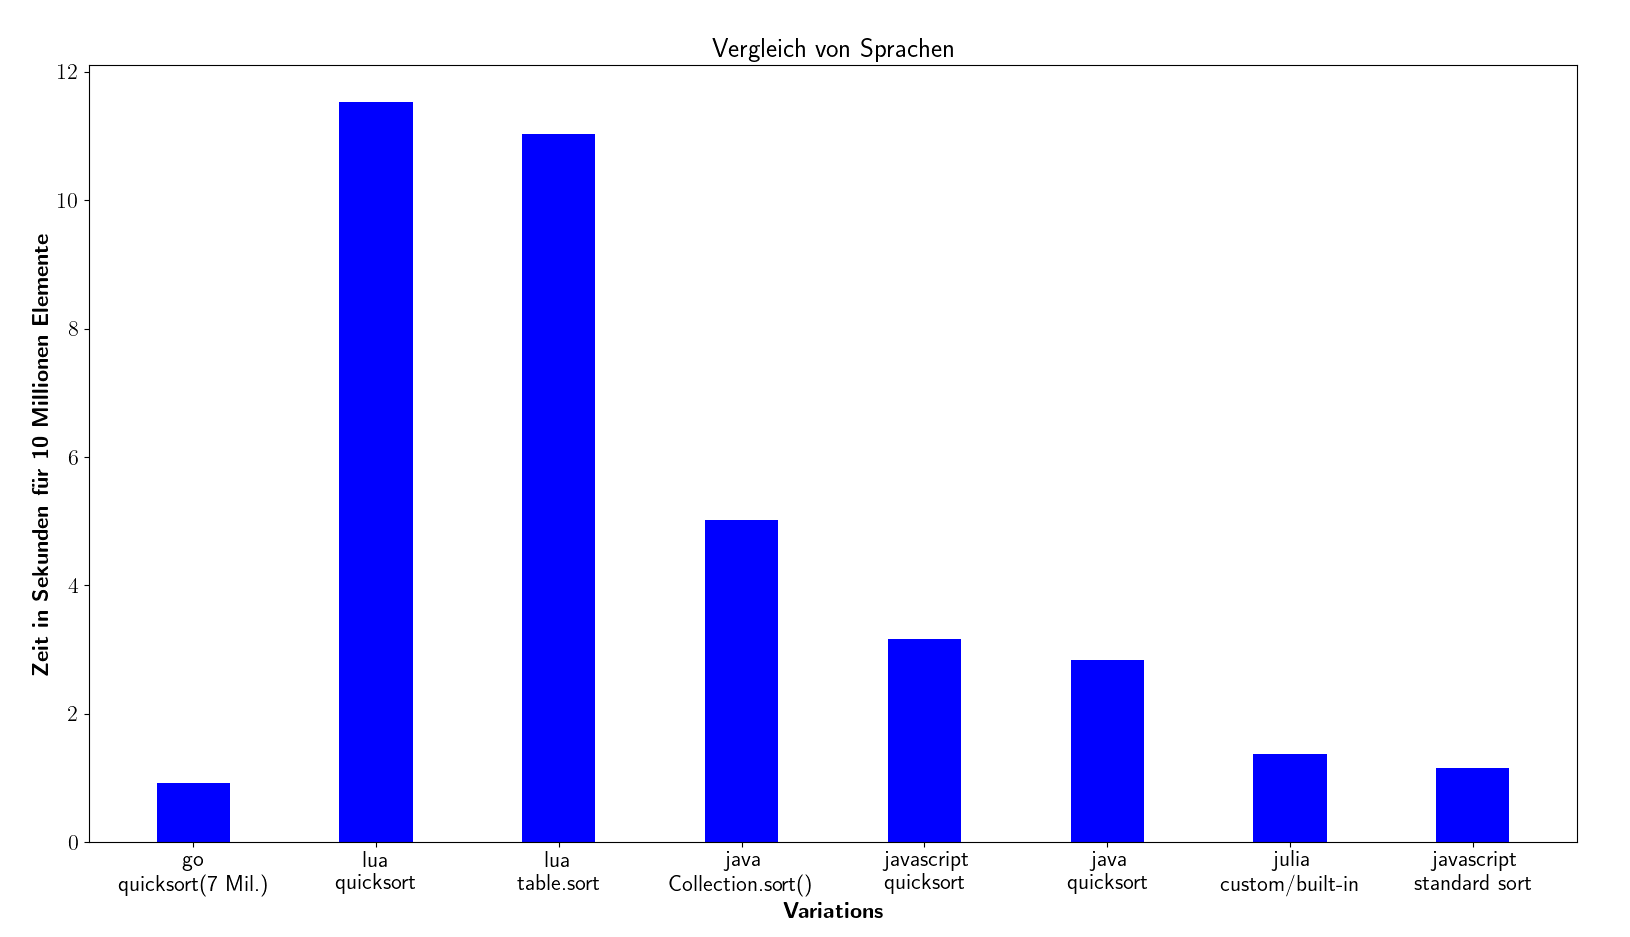
\includegraphics[width=1.2\textwidth]{./diagramme/matplotlib/comparison.png}
    Abb. 8 Großer Sprachenvergleich
\end{center}

\clearpage

Neben C++ und Python interessierte mich auch, wie schnell das Sortieren mit einer Implementation der Quicksort 
in anderen Sprachen möglich ist. Dazu testete ich 3 interpretierte Sprachen, nämlich Lua, Javacript und Julia sowie die
Kompilierten Sprachen Go und Java, wobei Java nur in Java-ByteCode kompiliert wird, der dann von der JVM ausgeführt wird.
Dabei stellte ich fest, dass Lua im Vergleich sehr langsam ist, doch die anderen interpretierten Sprachen ähnlich schnell zu Python waren.
Dies lässt sich dadurch erklären, dass die V8, also der Javascript Interpreter, im Gegensatz zum Python-Interpreter,
mehr Optimierungen vornimmt, so z. B. ohne Arbeit des Entwicklers direkt JIT-Compilation. Bei Julia hingegen hatte ich diese
schnelle Ausführung erwartet, da die Sprache für wissenschaftliche Berechnungen konzipiert ist. Obwohl man Julia Programme nicht selbst kompilieren kann,
so werden diese meist von der Julia Runtime vor der Ausführung kompiliert und optmiert, was zu dieser Performance führt.
Die Testergebnisse der beiden kompilierten Sprachen Java und Go sind leider nicht so aufschlussreich.
Bei Go hatte ich Probleme bei der Implementierung und durch die Unmöglichkeit, in Go eine echte, rekursive Quicksort mit 10 Millionen Zahlen
zu implementieren ist das Ergebnis nur Schätzbar. Ich würde die Geschwindigkeit ähnlich der wie Julia einschätzen, da 3 Millionen Zahlen weniger sortiert wurden.
Bei Java scheint sich auf den ersten Blick einer eher mäßige Performance abzuzeichnen, doch sollte man im Hinterkopf behalten,
dass ich sehr wenig Erfahrung mit Java habe, weshalb eine Implementation in Java möglicherweise schneller sein könnte.
Insgesamt zeigt sich, dass die Interpreter für Python und Lua nicht so gut optimiert sind, wobei man beachten muss, dass Projekte wie NumPy und Numba sowie LuaJIT
die Geschwindigkeit dieser deutlich erhöhen können.

\clearpage

\section{Diskussion}

Wie genau erklären sich diese großen Unterschiede in der Performance zwischen den Sprachen und vor allem innerhalb Python allein?
Warum sind C und C++ so schnell und was genau sind denn jetzt die Unterschiede zwischen Kompilierung und Interpretation bei Programmiersprachen.
Beim Python Interpreter, welcher in C programmiert wurde, gibt es grob gesagt 2 Arten, wie Code ausgeführt werden wird und
wie die Daten manipuliert werden. Normalerweise wird der Python Code vom Python Interpreter bei der Ausführung eingelesen und analysiert,
um die nötigen Operationen aus dem Code herauszulesen und diese dann auszuführen. Dies geschieht bei Python zur Laufzeit und läuft so ab,
dass mit dem Befehl 'python <pythonfile>' der Interpreter mit einer Input-Datei aufgerufen wird. Der Vorteil dabei ist, dass keine Kompilierung nötig ist,
doch deswegen gibt es meist Performance-Einbußen. Die andere Art der Code Ausführung ist die von nativ kompilierten C Funktionen,
die im Python Interpreter eingebaut sind und innerhalb von Python aufgerufen werden können. So wird die Ausführung dann von
bereits vorher kompilierten, stark optimierten C Funktionen übernommen, was zu hohen Geschwindigkeiten und mehr Effizienz führt.
Dieses Verhalten erschloss ich mir bei der Ausführung meines Codes und durch mein Vorwissen in diesem Bereich. Beweisen lässt sich
dies auch durch einen schnellen Blick in den Quellcode des Python Interpreters, wo sich die Implementation der "sort" Methode für Listen
finden lässt (in Objects/listobject.c, Line 2220) \cite{pythonsource}. Dies erklärt dann auch, wieso die normale Sortierfunktion in Python so gut abschnitt.
C und C++ hingegen basieren auf dem Konzept der "Ahead of Time" Kompilierung, also vor dem Ausführen des Programms.
Aufgrunddessen besteht zur Analyse des Quellcodes mehr Zeit und es können vom Compiler automatisch Optiemierungen vorgenommen werden.
Zusätzlich bestehen nach der Kompilierung alle Funktionen auf Assembler Befehlen bzw. Prozessorbefehlen und können somit 
also direkt vom Prozessor ausgeführt ohne den Schritt der in Python nötigen Interpretation.
Ein weiterer Grund, warum Kompilierung schneller ist, ist der Fakt, dass dabei das Programm genau auf den Prozessor zugeschnitten
werden kann. So können je nach Prozessor die besten Befehle ausgewählt werden. In Python hingegen ist dies nicht möglich,
da Programme bei der Ausführung im Textformat vorliegen müssen und die Ausführung generalisiert wurde, was im Gegenzug den Vorteil bringt,
dass einmal geschriebener Code von verschiedenen Python Interpretern auf gänzlich verschiedenen Systemen, also z. B. unter Windows und Linux,
ausgeführt werden kann, ohne dass Änderungen nötig sind.
Eine in Python nicht mögliche Optimierung für C++ ist z. B. AVX2, eine Möglichkeit, besondere Assemblerfehle
zu nutzen, die auf der Nutzung spezielle Hardware basieren, die in modernen CPUs verbaut ist 


\subsection{AVX2 Beispielcode}

\begin{center}
    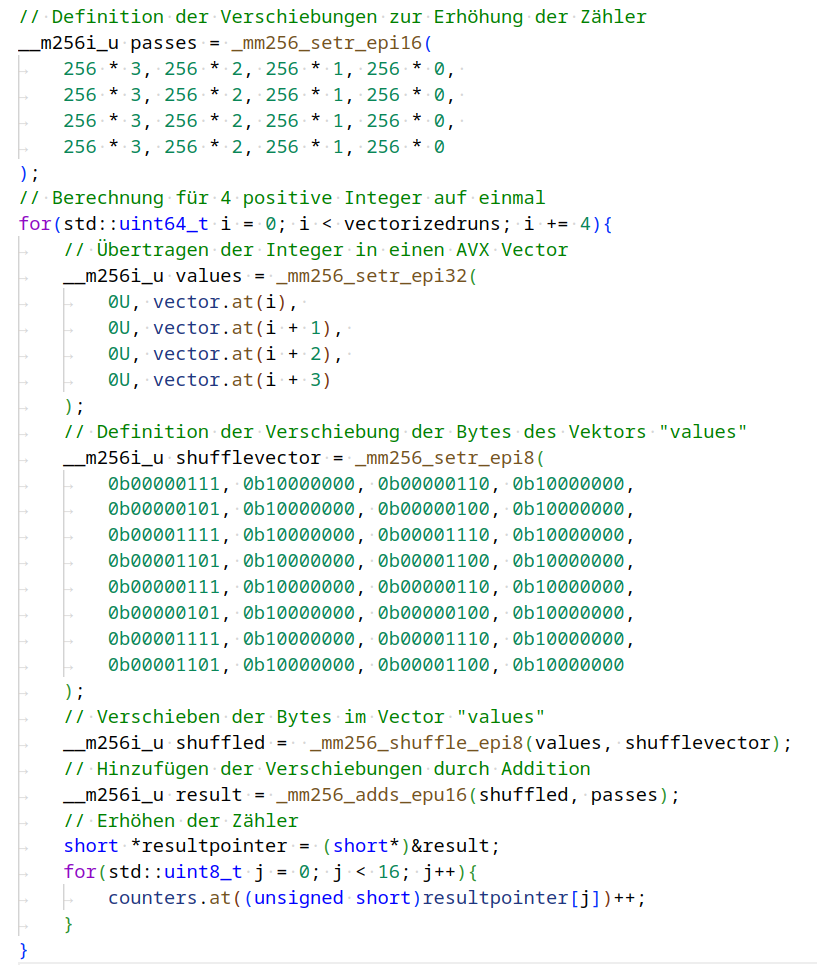
\includegraphics[width=1\textwidth]{./radix examples/avx2light.png}
    Abb. 9 Komplexer C++ Code mit AVX2
\end{center}

\clearpage

Dieser auf den ersten, und auch auf den zweiten Blick, komplex aussehende Ausschnitt von C++
Zeigt meine Verwendung von AVX2 zur bereits angesprochen Reduktion der Ausführung um 5 Millisekunden.
Es besteht ein starker Unterschied zu den meisten Programmen in Python, die deutlich einfacher
zu schreiben und zu verstehen sind, doch ich hoffe, dass zumindest einige dies nachvollziehen können 
(wer will, kann diesen Abschnitt überspringen).

\subsection{Erklärung AVX2 Beispielcode}

Einfach gesagt, teilt dieser C++ Code einen aus 32-Bit bestehenden, positiven Integer in 4 Teile auf und addiert
zu jedem dieser Teile einen Wert. Es werden dabei pro Schleifendurchlauf 4 Integer auf einmal geteilt, doch zum Verständnis reicht es,
den Prozess an einem Integer darzustellen.

\begin{center}
    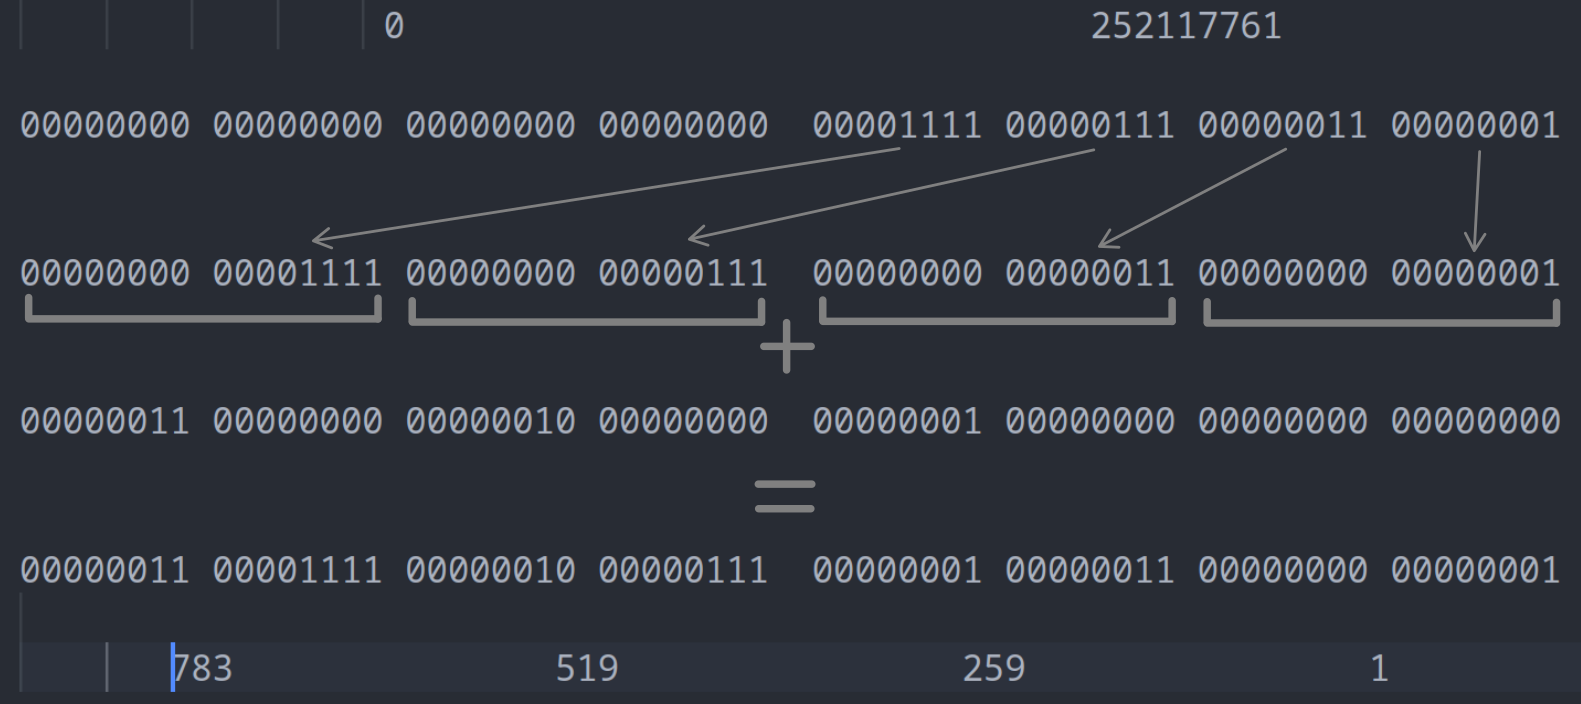
\includegraphics[width=1\textwidth]{./diagramme/matplotlib/avx2explanationfull.png}
    Abb. 10 Veranschaulichung AVX2 Integer Operationen
\end{center}

In Abbildung 10 ist der zu teilende Integer 252117761, der dort auch in binärer Form in der 1. Zeile
dargestellt wird. Zusätzlich gibt es vor diesem noch 32 Null-Bits. Im ersten Schritt werden nun die 4
Paare aus jeweils 8 Nullen oder Einsen, also jeweils 1 Byte, an eine andere Position der insgesamt 64-Bit bzw. 8
Bytes verschoben. Anschließend werden diese Bits, die man nun als 4 16-Bit sehen sollte (Spanne der grauen Markierung),
mit jeweils 4 anderen 16-Bit Integern addiert. Als Ergebnis hat man nun 4 16-Bit Integer, die
jeweils einer Position in dem 1024 Stellen langen Array entsprechen. An diesen Stellen wird nun der Zähler
um 1 erhöht.

\clearpage

\section{Zusammenfassung}

Während meinem Projekt fand ich heraus, dass die besten Möglichkeiten zur Optimierung in Python darin bestehen,
Numba und NumPy zu nutzen und dass Cython nicht ganz mit den möglichen Performance-Steigerungen der beiden Bibliotheken mithalten kann.
Außerdem stellte ich fest, wie stark Python zur Ausführung schneller Programme auf C Code aufbaut und wie stark das Zusammenspiel dieser
beiden Sprachen ist.
Bei meinen Abenteuern mit C++ musste ich dann erfahren, dass durch schlechte Implementierung eines eigentlich überlegenen Algorithmus sich die
Performance auch deutlich verschlechtern, wobei ich gleichzeitig auch sah, wie durch korrekte Implementation sich die Geschwindigkeit drastisch
erhöhen kann. Schlussendlich schaffte ich es auch, komplexe Optimierungen wie AVX2 zu nutzen, um noch das letzte Quäntchen Performance zu gewinnen.
Insgesamt würde ich sagen, dass es mir gelungen ist, herauszufinden, wie sich schneller Code schreiben lässt und worauf man achten soll.
Auch lernte ich viel über die zugrunde liegenden Konzepte.
Besonders Mindblowing finde ich die Erkenntnis, dass sehr viele Sprachen stark auf C/C++ Code aufbauen
und die effizienten, in diesen Sprachen implementierten Algorithmen, Programme und Bibliotheken, dass ganze System
der Programmiersprachen stützen und somit auch indirekt unsere digitale Welt.
Ein Beispiel dafür ist zum Beispiel das hochaktuelle Thema Künstliche Intelligenz und neuronale Netze.
Dort ist die meist genutzte Sprache zwar Python, doch in diesem Fall ist Python, wie in vielen Fällen, nur
eine Möglichkeit, ursprünglich in C/C++ geschriebenen Code aufzurufen und zu nutzen.

\section{Schlusswort}

Alle, die Performanten und Schnellen Code schreiben wollen, sollten sich über die Funktionsweise ihrer 
Software und ihrer Bibliotheken genauestens informieren.
Alle, die neue Algorithmen und komplexere Bibliotheken entwickeln wollten, sollten C/C++
Verwenden, aufgrund der erstklassigen Performance und der Einbindung in fast alle Sprachen.

\clearpage

\printbibliography[title={Literaturverzeichnis}]

\end{document}
